\documentclass[a4paper,10pt,onecolumn]{article}
\usepackage{graphicx} % Required for inserting images
\usepackage{xcolor}
\usepackage[english]{babel}
\usepackage[utf8]{inputenc}
\usepackage[left=1.6cm,text={18cm, 24.7cm},top=1cm]{geometry}
\usepackage[normalem]{ulem}
\usepackage{amsmath} 
\usepackage{amssymb} 
\usepackage{hyperref}
\usepackage{multicol}

\hypersetup{
    colorlinks=true,
}

\title{ISCTE - Statistics 1}
\begin{document}

\maketitle

\section{Introduction}
Email: pnsoa@iscte-iul.pt
\\Statistics for business and economics newbold \href{https://handoutset.com/wp-content/uploads/2022/07/Statistics-for-business-and-economics-Paul-Newbold-William-Lee-Carlson-etc..pdf}{pdf}
\\ Khan academy on \href{https://www.youtube.com/@khanacademy}{yt}
\section{Descriptive statistics}
\subsection{Topics}
\begin{itemize}
  \item Types of variables
  \item Frequency
  \item Central Tendency Measures
  \item Dispersion measures
  \item N.C.T measures
\end{itemize}
\hrule % Horizontal rule

\subsection{Types of variables}
\begin{multicols}{2}
\subsubsection{Qualitative}
\textbf{Nominal variable}
\\Type of categorical variable where the categories represent distinct groups with no inherent order or ranking
\begin{itemize}
   \item Blue
  \item Brown
  \item Green

\end{itemize}
\textbf{Ordinal variable}
\\Type of categorical variable where the categories have a meaningful order or ranking
ordinal variable 
\begin{itemize}
  \item High School Diploma
  \item Bachelor's Degree
  \item Master's Degree 
  \item Doctoral Degree 
\end{itemize}
\columnbreak
\subsubsection{Quantitative}
\textbf{Discrete variable}
\\Variables are those that can only take on specific, distinct values and cannot be divided into smaller units.
\begin{itemize}
    \item Number of cars in a parking lot (0, 1, 2, 3, ...)
\item Number of students in a classroom (0, 1, 2, 3, ...)
\end{itemize}
\vphantom{\textbf{Continuous variable}}
\\\textbf{Continuous variable}
\\Variables represent data that can take on an infinite number of values within a given range.
\begin{itemize}
    \item Temperature measured in degrees Celsius or Fahrenheit is a continuous variable. It can have decimal values, and there are infinite possibilities within the temperature scale
\item Human height. It can vary continuously from the shortest to the tallest individuals, and there are infinitely many possible height values within a specific range.
\end{itemize}
\end{multicols}
\subsection{Frequency}
\subsubsection{Frequency table}
A frequency table is a table that displays the number of outcomes of a sample that fall into different categories. The categories are usually specified in the first column, and the frequencies are specified in the second column. The frequency of a particular category is the number of times the data value occurs in the data set.
\\
\textbf{Legend:}
\begin{itemize}
    \item $X_i$ = Value of the variable
    \item $F_i$ = Frequency of the value
    \item $f_i$ = Relative frequency of the value
    \item $cumF_i$ = Cumulative frequency of the value
    \item $cumf_i$ = Cumulative relative frequency of the value
  \end{itemize}
\begin{figure}[h]
    \centering
    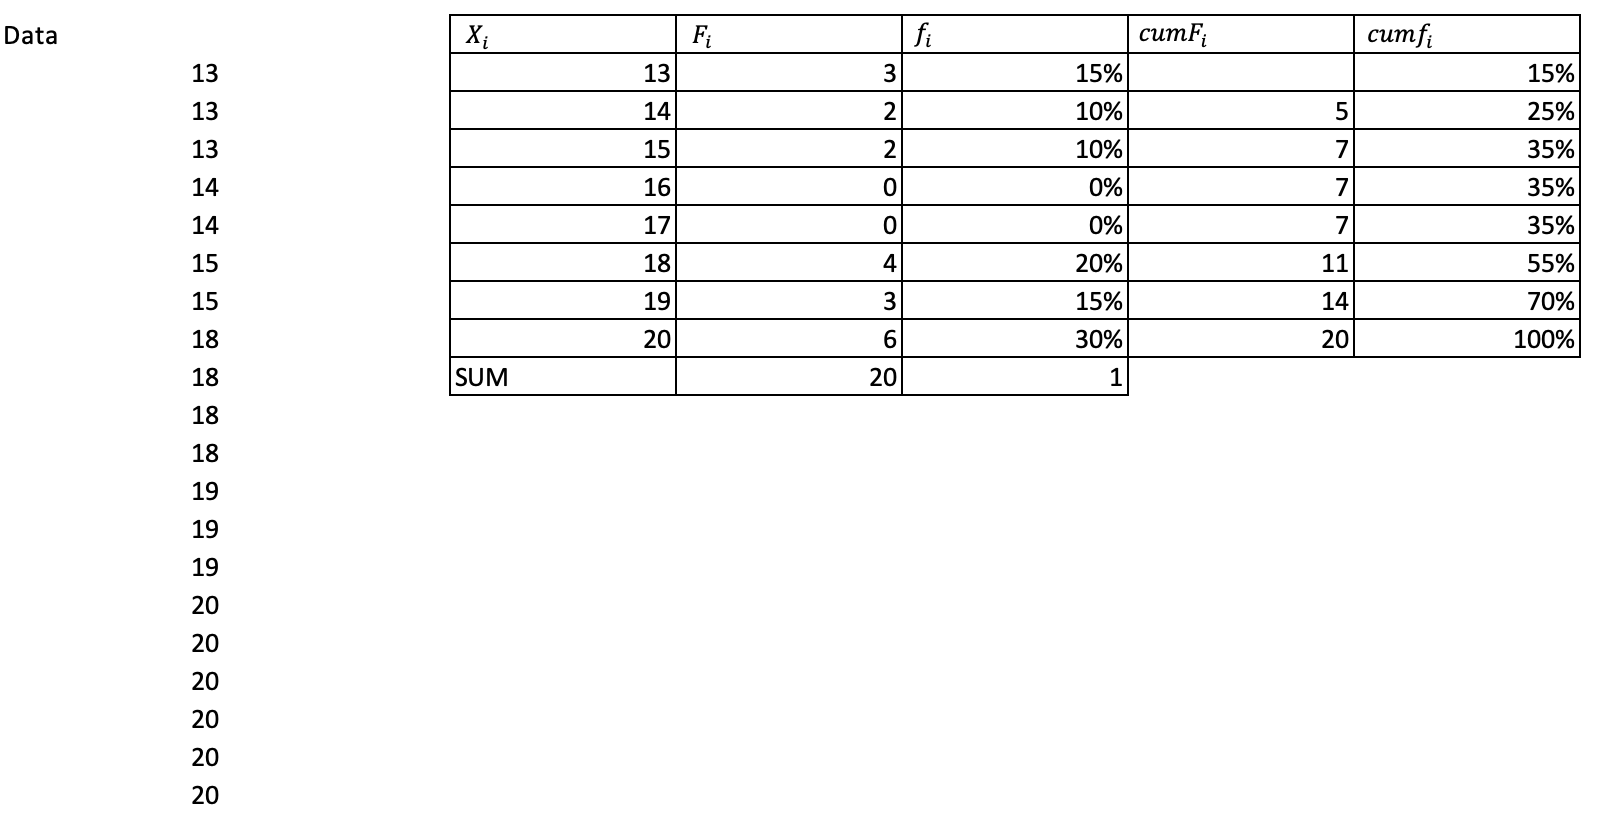
\includegraphics[width=\textwidth]{freq.png}
    
  \end{figure}
  \newpage
\subsection{Mean, median and mode }
\subsubsection{Mean}
The mean, often referred to as the average, is calculated by adding up all the values in a data set and then dividing the sum by the total number of values. It provides a measure of central tendency and represents the "typical" value in a data set.
\\
\textbf{Mean} = (Sum of all values) / (Number of values)
\subsubsection{Mode}
The median is the middle value in a data set when it is arranged in ascending or descending order. To find the median, you first arrange the data points and then identify the middle value. If there is an even number of values, the median is calculated as the average of the two middle values. The median is less affected by extreme outliers compared to the mean, making it a robust measure of central tendency.
\subsubsection{Mode}
The mode is the value that appears most frequently in a data set. Unlike the mean and median, which focus on the central tendency, the mode highlights the most common value(s) in the data. A data set can have one mode (unimodal), multiple modes (multimodal), or no mode at all if all values occur with equal frequency.
\\
\subsubsection{Example}
\begin{figure}[h]
    \centering
    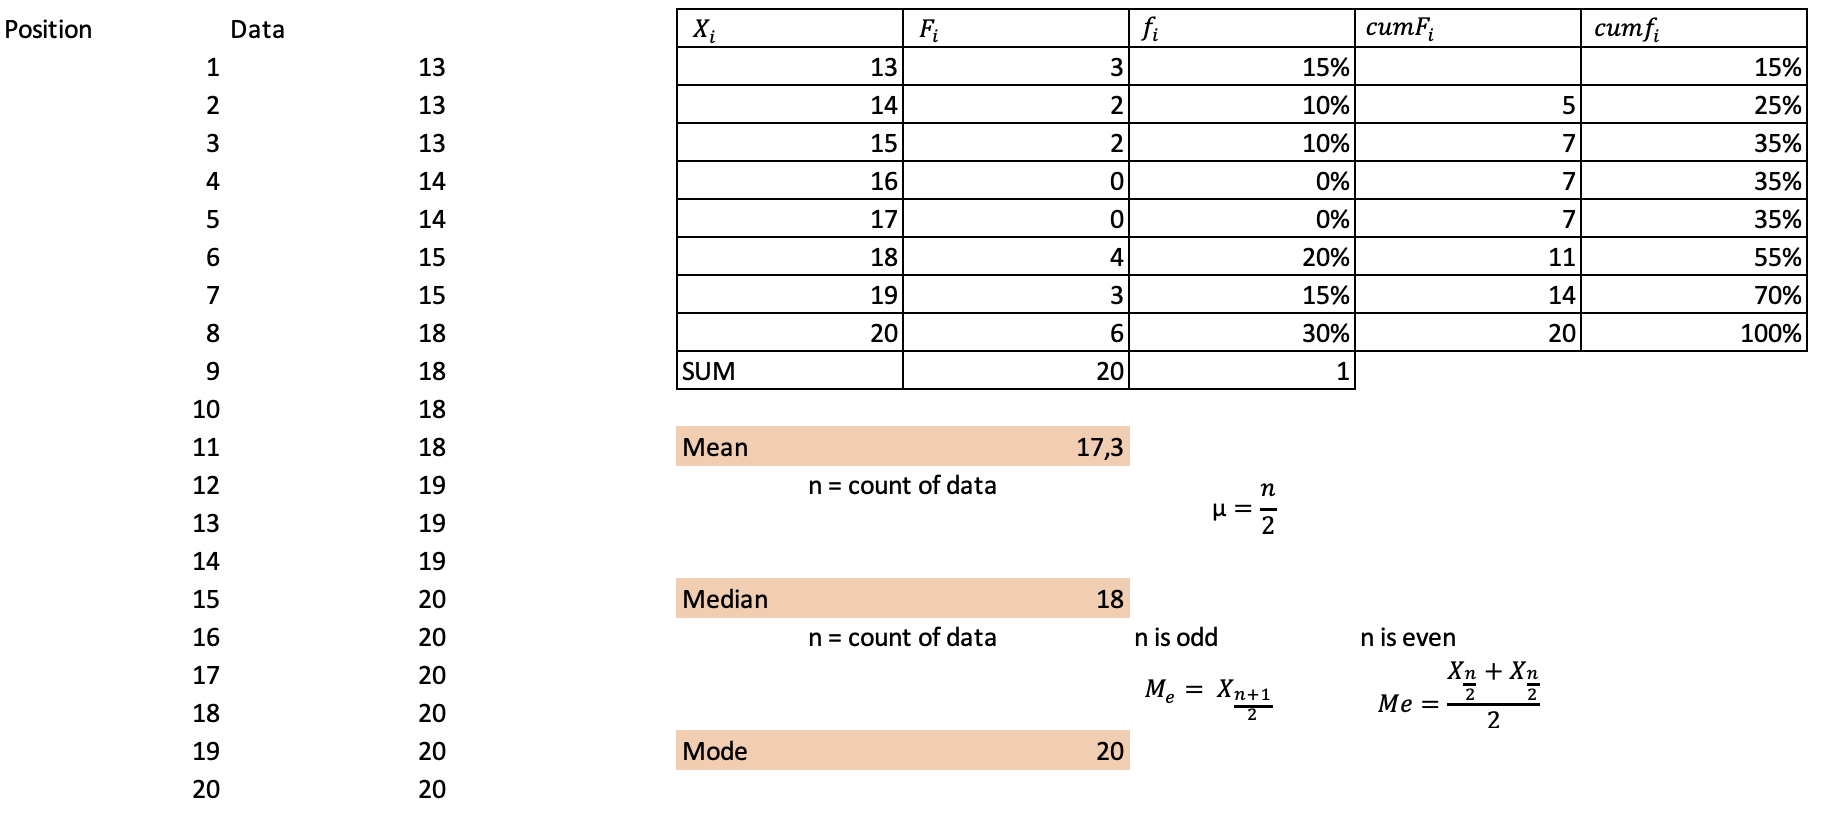
\includegraphics[width=\textwidth]{mmm.png}    
\end{figure}
\subsection{Quantiles}
\subsection{Variance dispersion}


  
\end{document}
